\pagestyle{fancy}
\chapter{Grid integration}
\label{chp:grid}
%\pagenumbering{arabic}

Computational power is cheap. Storage is also cheap and networking as well.
A well known empirical law for the increase of processing power is the Moore's law
\cite{moore-law}, which dictates the doubling of computational speed every
18 months. Similar laws have been envised for networking (doubling every 9
months) and storage capacity (doubling every 12 months). For scientific
needs, computational power and storage often are the limiting factors
for new developments and insights. 

The dramatic increase of networking performances opens new possibilities to
obtain computational power and storage from unused or underutilized
resources.  This deploys the fundation of a new paradigm for distributed
computing: grid metasystems.  Using grids, it is possible to pool
\begin{itemize}
\item \textit{Fabric resources}, like disk space, computational power, RAM storage,
data aggregation and archiviation, instruments
\item \textit{Logical resources}, like experimentation, data analysis, modeling,
simulation
\item \textit{Human resources}, like competence sharing, administrative burden,
communication.
\end{itemize}
The result is a distributed, heterogeneous metasystem, which provides a
virtual structure to the end user.  Interaction with services is
standardized and uniform, regardless of differences like CPU architecture
or geographical location. In this panorama, a grid provides
virtually infinite resources ready to use to produce a better science.

The most famous example of a grid is probably the Web. The well-known WWW is
a very simple storage grid where documents and informations are
geographically distributed. Users can access these informations through a
well-known interface (a web browser) which makes use of a low-level
uniform protocol (HTTP\cite{http-site}) in order to access resources.
The abstraction provided by the Apache webserver\cite{apache-site}
translates the HTTP requests into fabric level access, like reading or
writing a given file, or running a script.

Consortiums like IETF\cite{ietf-site}, W3C\cite{w3c-site} and
OASIS\cite{oasis-site} ratified standards in order to define
guidelines from low-level issues to high-level protocols and interactions:
TCP/IP\cite{tcp-site,ip-site}, HTTP, XML\cite{xml-site},
SOAP\cite{soap-site}, WSDL \cite{wsdl-site}, UDDI \cite{uddi-site}, RDF
\cite{rdf-site}, WSFL \cite{wsfl-site} are some examples of these standards.
Toolkits, frameworks and utilities have been developed, both commercial and
opensource to exploit the grid paradigm: Legion \cite{legion-site}, Globus
\cite{globus-site,ogsa-site}, and Unicore \cite{unicore-site} are some examples.

At the moment, a restricted set of grid applications can be devised:
\begin{itemize}
\item \textit{Low communication applications}: also known as ``embarassingly
parallel'' applications. For these applications, the problem is decomposed in
small almost independent pieces (usually called \textit{Working Units}),
and the computation is carried over each working unit. This category is
well represented by Seti@Home\cite{seti-site} or weather analysis
\item \textit{Staged applications}: the procedure is decomposed in
serialized steps, each one performed on a given site on the grid. This
approach is useful to manage human factors, like competence sharing and
administrative burden, license problems, use of private code, security
reasons
\item \textit{Resource access}: a resource from a service provider is made
accessible by request. Classic examples could be databases, instruments,
storage farms.
\end{itemize}

For quantum chemical processes some experience has been made, mainly with
parallelization of various algorithms (using PVM \cite{pvm-site}, MPI \cite{mpi-site} or OpenMP
\cite{openmp-site}). However, quantum chemistry evaluations are mainly
serialized in nature: for \textit{ab initio} calculations, a step involving
the evaluation of integrals is followed by other treatments, which in turn
provide information for others and so on.  This calls for a ``Staged
application'' architecture. This architecture is also enforced by
administrative issues, competence sharing and license problems, and finally
a current intrinsic complexity in the creation of multiplatform codes.

\section{Metachem grid}

The Metachem grid is a project for producing ``a meta-laboratory for code
integration in \textit{ab initio} methods''. The project, still in
development, has been carried on under the D23 COST action \cite{cost-site},
with the objective to develop a common grid infrastructure where
computational chemists can access several \textit{ab initio} codes produced
by different laboratories through a simple and user-friendly interface.

Most of the interested parties developed quantum chemistry codes for
{Post-SCF} evaluations, mainly for internal research. These techniques can be
integrated in a common infrastructure, but with the requisite to leave each code
on the platform it was originally designed for, under the responsibility of
its owner for maintenance and production. This will distribute the
administrative burden and avoid binary code duplication.

Finally, a set of standard quantum chemistry codes (\texttt{MOLCAS},
\texttt{COLUMBUS} or \texttt{DALTON}) must be integrated into the grid to
provide commonly used entities, like integrals, overlap, CASSCF orbitals and
wavefunctions, and so on.

Various considerations, ranging from technical factors to license
restrictions prevent direct changes to existing codes. A more conservative
strategy has been considered, at least in the initial deployment of the
project (see Fig.~\ref{fig:wrapper-scheme}): input and output wrappers
convert files and workflow logic between the local environment of a given
program and the shared grid environment, and viceversa. Input wrappers
convert information provided by the grid to low-level input such as Fortran
namelists and proprietary binary files. Output wrappers parse the products
of the program and create the standard information which will return to the
grid.

\begin{center}
\begin{figure}[ht]
\begin{center}
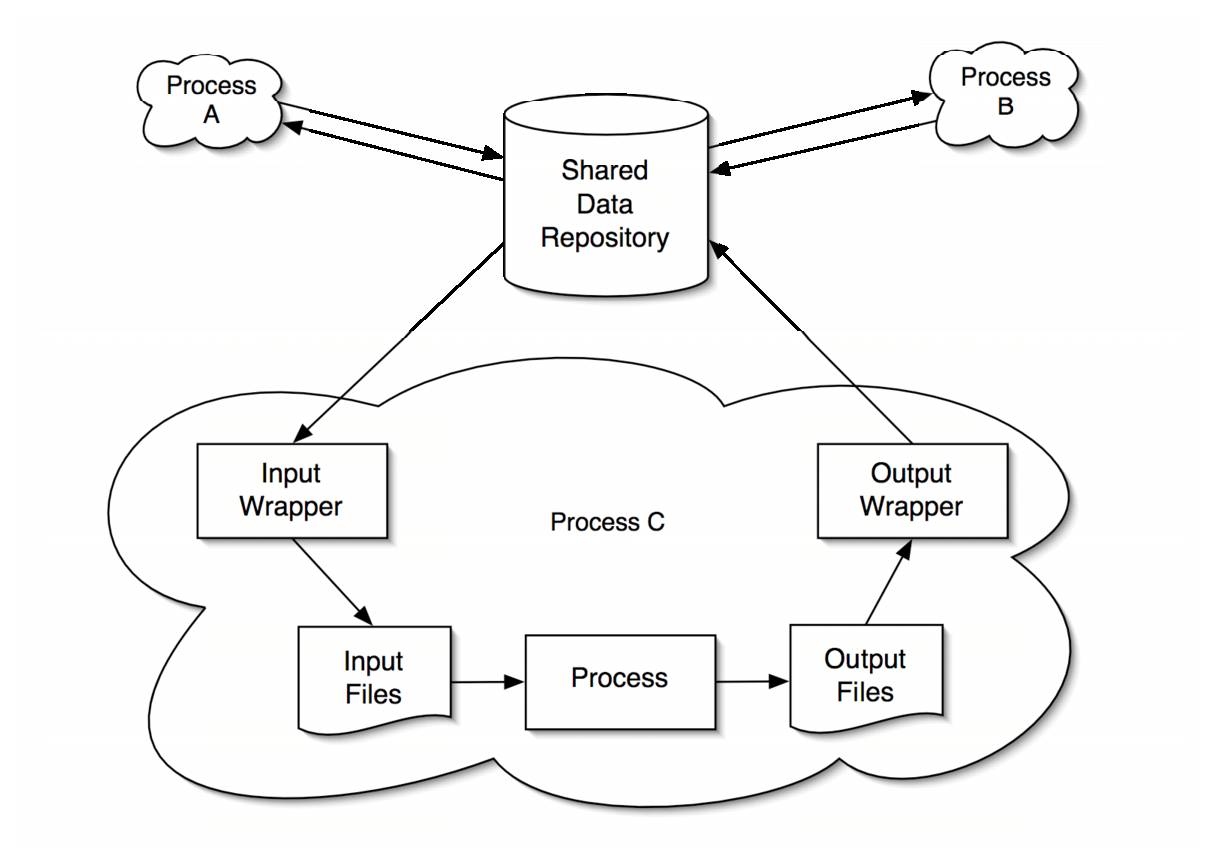
\includegraphics[width=10cm,keepaspectratio]{04_grid/images/wrapper-scheme-gimped.eps}
\end{center}
\caption{\footnotesize A scheme for the data handling inside a single
calculation environment. Data are made available by the data repository,
adapted to the local input environment of the process. The result is
converted back to the standard format and returned to the repository.}
\label{fig:wrapper-scheme}
\end{figure}
\end{center}


This strategy imposes the development and maintenance of the wrappers by
the interested parties. They are supposed to track the changes of their own
codes and adapt the wrappers accordingly. For historical reasons,
the reference language for the development of these wrappers is Fortran. 

The shared environment must also agree on a common file format.  Due to the
nature of the project, this common file format must be platform independent,
code independent, and easy to debug. Two different kinds of information have
been identified in quantum chemistry calculations:
\begin{itemize}
\item \textit{small data}, mainly ASCII encoded, like atom labels, geometry,
symmetry, basis sets, but also workflow specific information
\item \textit{large data}, normally binary encoded, like integrals and expansion coefficients
\end{itemize}

For the first kind of data, many initiatives are active nowadays. The more
extensive is the work of Murray-Rust et al.\cite{jcics-39-928-1999,
jcics-41-1113-2001,jcics-41-1124-2001,cc-1471-2000,njc-618-2001} with the
development of CML (Chemistry Markup Language) under the eScience project in
UK. The choice of XML allows both human readability and machine parsing.

Unfortunately, CML does not provide direct support for quantum chemical
entities.  After a brief analysis of the problem, an experimental
\textit{XML-schema} for quantum chemistry entities, QCML (Quantum Chemistry
Markup Language) has been deployed. The parsing of this information in
Fortran is possible through a library, named F77/F90xml, specifically
developed for the project.

For the second kind of data (large binary data) XML is not a good
technology, mainly due to its verbosity. For several reasons,
HDF5\cite{hdf5-site} is considered the best technology for large binary
data.

The next step, to be done in the future, is the definition and setup of
user defined workflows based on heterogeneous codes, located on different
platforms, communicating through the common formats. The actual technology
has yet to be chosen, but the choice seems to be oriented towards
UNICORE\cite{streit-tbp-2005,erwin-unicore,unicore-site}, together with a
common language for describing both workflow and intrinsic differences
between work paths. 

The final infrastructure is expected to satisfy both grid requirements
(fault tolerance, reliability) and human interface requirements (access via
web interface or specialized clients). An access point to grid services will be provided by
the CINECA supercomputing center. Its role is to coordinate the federated
system, where each node provides one or more services to the grid.


\section{Q5Cost library}

In the deployment of a common suite of codes, a standard file format is
necessary.  A first attempt in file standardization has been made in
Toulouse with the COST format. This format has been also implemented in most
of the Ferrara suite.

The format is made of four files, each one with a different extension:
\begin{itemize}
\item \texttt{.Mono}, a binary file containing the atomic basis set overlap and the one-electron
integrals on the molecular orbital basis set
\item \texttt{.ijcl}, a binary file containing the two-electron integrals
on the molecular orbital basis set
\item \texttt{.Info}, a cleartext file containing namelists describing various
metainformation, like the number of active orbitals, the nuclear
repulsion energy, the geometry and so on
\item a file called \texttt{INPORB}, containing the molecular orbitals. The format is
the same provided by the \molcas program, enriched with additional
information needed by the Toulouse suite of programs.
\end{itemize}

The COST files are written using the standard sequential access provided by
\texttt{READ} and \texttt{WRITE} statements in Fortran. No
{intention-revealing} interfaces are provided for accessing the data. This
implementation, although simple to manage, is limited in a lot of points:

\begin{itemize}
\item the standard sequential access provided by Fortran imposes to agree
on data size, data ordering, and chunking. It does not allow random access,
making difficult to update already written information, or to posticipate
the writing operation of some entity. It complicates reorganization
or expansion of the stored information set
\item files are not platform independent. A file written on an Intel
x86 machine is unreadable by an IBM SP4 supercomputer, and viceversa. This
limits the output sharing
\item it is difficult to access the stored information in a clear
representation. This is a major issue when debugging computational chemistry
codes. At the moment the access is through ad-hoc visualizers or hexadecimal
editors
\item the file is difficult to split, merge, compare, or describe with
metainformation
\item the API for accessing the file format is limited in features,
allowing no basic consistency checks or a clean interface. Documentation 
is written as code comments. This makes difficult to direcly access the
information.
\end{itemize}

Q5Cost is a library devoted to solve these problems. Based on the
{platform-independent} file format HDF5, Q5Cost allows the user to produce binary
files through a well documented interface. The library also takes care of
providing useful information during debug, explicitly stating inconsistent
data or wrong usage of the routines.

\subsection*{HDF5 file format}

As defined on the website\cite{hdf5-site}, ``HDF5 is a general purpose library and file
format for storing scientific data''. HDF5 targets the data management needs
of scientists and engineers working in high performance, data intensive
computing environments. This is achieved by providing an efficient library and
file format, specifically tuned to read and write binary data efficiently.

A HDF5 file appears to the user as a single file containing a structured
graph of entities. This structure is conceptually very similar to a UNIX
filesystem, and is defined by means of three entities: \textit{Groups},
similar to directories, \textit{Datasets}, similar to files
and \textit{Attributes}, similar to metainformation such as permissions and
owner.  Data are stored into Datasets and Attributes, and can be organized
with Groups. The HDF5 library provides an interface to handle these
entities.

The most striking feature of HDF5 is the platform independence of the files.
A file written on a 32 bit Little Endian architecture (like, for example, an
Intel x86 machine) can be transferred and read transparently on a 64 bit Big
Endian machine (like, for example, the IBM SP4) or a 64 bit Little Endian
machine (like an IA64 machine). This is of critical importance
in grid environments, where heterogeneity is the rule, rather than the
exception.

Another important feature of HDF5 is the suite of utilities, which allows the
user to find differences between two HDF5 files, obtain a textual dump of
Groups, Datasets and Attributes layout (resembling the ``ls'' program in
UNIX environment) or a more detailed view presenting also the numerical
data.  This simplifies the access to this information, which is critical
in the debug phase.

The HDF5 library is made of a directly accessible C layer. Alternative APIs
are available for C++, Fortran 90, and Java. The library is actively
developed, is free and released as open source software.

\subsection*{Q5Cost file format and library} 

The Q5Cost library is implemented on top of the HDF5 library.  It provides
read and write access to HDF5 files with a specifically designed high-level
interface for quantum chemistry developers. 

The rationale is to provide a Fortran interface based on well known chemical
entities, rather
than groups or datasets like in the HDF5 interface. HDF5 takes care of
low-level management of the file, and Q5Cost provides the high-level
API to store and retrieve chemical entities.

An extensible data model has been rationalized thanks to the knowledge
obtained by the involved researchers. Some firm points have been
discovered.

The first point is that many different types of simple and small data
must be handled. Some examples are nuclear energy, molecular orbital labels,
molecular symmetry and so on. We will refer to these data as
\textit{metadata}, in order to distinguish them from the real large
information on the chemical system, the integral values.

Metadata represents well-known chemical entities and belong to three
generic data classes: \textit{Scalars}, \textit{Vectors} and
\textit{Matrixes}. For example, the nuclear repulsion energy is a floating
point scalar, molecular orbitals can be represented as a (N,M) floating point matrix, the
associated orbital energies is a floating point vector, the molecular
orbital labels is a vector of strings and so on. The library should provide
an interface for accessing these data, both as generic or specialized
entities.

A second point is the fact that in quantum chemistry large sparse
matrixes with an arbitrary number of indexes (rank-$n$ arrays) are very
common data structures. These data usually scale aggressively with the
system size, and they are normally accessed with a chunked sequential approach.
This is the case of entities like two-electron integrals, or atomic
orbitals overlap, but also much other more application-specific
information, like the four-particles density matrix.

The sparse nature of these matrixes encourages to store only non-zero
elements, each one associated to $n$ indexes in the case of a rank-$n$
array. This representation of the data, although not always efficient in
term of space occupation, is well known by the interested parties, easy to
debug and already integrated in the current codebase both for memory
representation and file storage. The library structure allows 
future expansions of the low-level storage format, in order to reduce the
storage needs, but in the first development phase this issue has not
been investigated, and the current format is useful for the direct debug of
the file.

These large data arrays share common features:
\begin{itemize}
\item they usually are integrals, whose evaluation involves one
operator and a given number of functions. These functions are
referred by the indexes of the matrix. For example, two-electron integrals
on the molecular orbital basis are stored as a rank-4 array with indexes
referring to the molecular orbitals. In the case of atomic basis set overlap
integrals, the indexes refer to the atomic basis set
\item the rank of the array depends on the physical meaning of the
integrals. Atomic basis set overlap is described by two indexes, and can be
stored as a rank-2 array. Two-electron integrals have four indexes imposing a
rank-4 array and the four-particles density matrix has eight indexes,
requiring a rank-8 array
\item additional information is needed to describe the involved operator
(for example its symmetry) and the entities the indexes refer to.
\end{itemize}

All this information can be classified under a generalized \textit{Property}
concept, which is described by the matrix rank and the definition of the
involved operator and functions. Integrals are stored by means of a
dedicated abstraction, named \textit{CompactMatrix}, enriched with
metadata to define the Property, like its name, rank, symmetry and
real/complex nature.

Some properties are well-known chemical entities, and chemists are
used to refer to them by name. A specific library access has been provided
to handle these entities, easing the need to specify well-known information
about them.

A further step is to recognize containment relationships and simple
consistency patterns between the involved entities. A graphical
representation can be seen in Fig. \ref{fig:q5cost-schema}.

\begin{center}
\begin{figure}[ht]
\begin{center}
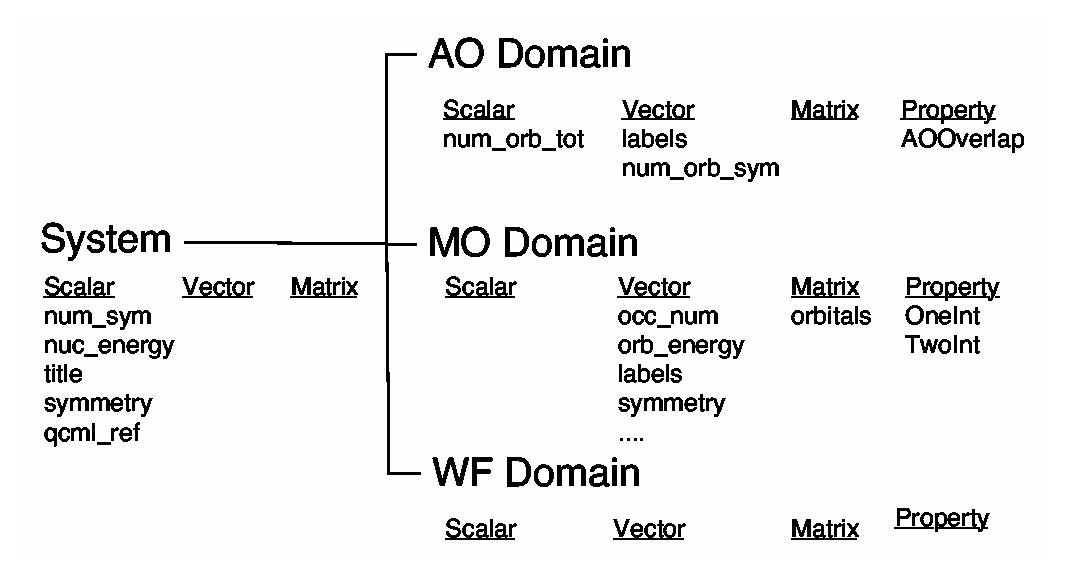
\includegraphics[width=10cm,keepaspectratio]{04_grid/images/q5cost-schema-gimped.eps}
\end{center}
\caption{\footnotesize A graphical representation of the containment
relationship between the System and the Domains. Specific metainformation is also
presented, classified under the appropriate environment.
}
\label{fig:q5cost-schema}
\end{figure}
\end{center}


The first high-level logical container is the \textit{System} object. This
object represent a molecular system as described by its structural
informations, such as symmetry and atomic coordinates, and also contains all
the metadata that are invariant at this level, like for example nuclear
repulsion energy, or a title. Multiple Systems make possible to handle
different molecular geometries.

A System can contain several \textit{Domains}. The role of a Domain is to
group together Properties whose indexes conceptually refer to the
same entity. Three Domains have been recognized as fundamental: \textit{AO}
for Atomic Orbital, \textit{MO} for Molecular Orbitals and \textit{WF} for
Wavefunction.  Each Domain can contain an arbitrary number of Properties, and
additional metadata represented as specialization of Scalar, Vector and Matrix
entities.

The AO Domain holds Properties whose indexes refer to the atomic basis set
funtions: overlap, one-electron and two-electron integrals on the atomic
basis set are some examples, in addition to the generic Property. The
associated metadata hold information about the atomic orbitals, like their
number, labels and symmetry.

The MO Domain holds Properties referring to molecular orbitals:
one-electron and two-electron integrals on the MO basis set are examples, in
addition to the generic Property. The descriptive metadata refer to the
molecular orbitals, their number, labels and symmetry, the AO
basis they were derived from, orbital energies, classification and
occupation numbers.

The WF Domain holds Properties referring to the electronic states. At the
moment a complete definition of this Domain is not available and not
subjected to major research and development, given its non-critical nature
for the first deployment of the library.

Each Domain can be defined under different occurrences, by means of a textual
identifier (\textit{tag}) chosen by the user, with a default value if no tag is
provided. The aim is to provide storage of multiple entries for each Domain,
like in case of multiple molecular orbitals in the MO Domain, or multiple
basis sets in the AO Domain.

\subsection*{Library structure}

The library is written in Fortran 95 and is made of different modules, each
one providing different facilities. The most important modules are

\begin{itemize}
\item \textit{Q5Cost}: defines the high-level API, providing
subroutines designed to be accessible from the final programmers of the
laboratories involved in the project
\item \textit{Q5Core}: provides a wrapping facility for HDF5 routines, in order to
perform additional useful services like reference counting and debugging.
Also provides simplified routines to perform frequently used low-level
tasks
\item \textit{Q5Error}: provides facilities for high-level debugging of the
library and client codes. This module implements a ring buffer for error
messages, different logging levels, generic reference counting for catching
leaks of HDF5 references, and a subroutine call stack trace.
\end{itemize}

Subroutines for each module have been namespaced with an appropriate prefix,
and names have been chosen to provide an explicit and {intention-revealing}
interface to the entities described in the previous section.  

Although Fortran 95 does not allow object oriented (OO) programming, some OO
concepts have been used in the development of the library, keeping into
account the procedural programming background of the final developers. The
state is preserved into the HDF5 file, and subroutines refer to the file
directly through the HDF5 identifier, a more easy concept for Fortran
programmers used to unit descriptors.

\subsubsection*{The Q5Cost module}

This module is the main reference for the final users. It provides
subroutines to read and write HDF5 files in the Q5Cost format with a high-level
abstraction. The users can deal with high-level concepts without worrying
about low-level implementation details. If a finer access is needed to the
underlying HDF5 file, the Q5Core module provides this access in a simpler
way with respect to raw HDF5 routines.

The Q5Cost module is made up of routines belonging to the following
classes:
\begin{itemize}
\item \textit{File}: create, open, close the file and write/read root
metainformation, like creation time, access time and file version
\item \textit{System}: create or check the existence of the System and set/get
its metainformation
\item \textit{AO}: create or check the existence of the AO Domain and set/get its
metainformation
\item \textit{AOOverlap}: create, read and write data for the atomic basis set
overlap Property
\item \textit{MO}: create or check the existence of the MO Domain and set/get its
metainformation
\item \textit{MOOneInt}: create, read and write data for the one-electron
integrals in molecular orbitals basis
\item \textit{MOTwoInt}: create, read and write data for the two-electron
integrals in molecular orbitals basis
\item \textit{WF}: create or check the existence of the WF Domain and set/get its
metainformation. Still experimental and mostly unimplemented.
\end{itemize}

Additional routines are provided for generic access to the Property
class, allowing to manage generic property data. Subroutines for
AOOverlap, MOOneInt and MOTwoInt delegate calls to these Property routines,
automatically passing well-known parameters about the involved property.

Q5Cost module routines provide a context-based access to chemical
entities. This access is transformed into a path-based access, creating
an appropriate layout for HDF5 groups, datasets and attributes, and
writing the user-provided data on the file. Some data are automatically
written by the library, like the creation or access time and the
Q5Cost library version. 

One important aspect of this format is that the user is not forced to
produce information for all quantities. The user can store only those
quantities that are actually available.  Constraint checks are however
mandatory in order to assure basic file consistency. For example, no MO
Domain can be created if a System and an AO Domain have not been provided,
in order to guarantee the presence of fundamental data, like the number of
symmetry species and the number of basis functions for each symmetry
species.

\subsubsection*{The Q5Core module}

The Q5Core module is a low-level module designed to provide wrapping
facilities between the Q5Cost library and the HDF5 library. At the moment it
is focused at providing additional debug information, reference counting
for HDF5 objects, additional low-level API to simplify common tasks.

This module also provides path-based creation of Scalar, Vector and
Matrix entities (in contrast with the context-based approach of the Q5Cost
module, which focuses on chemical concepts rather than HDF5 paths) and also
routines to ease handling of the Property index/value data, relative to the
CompactMatrix class. Most of the Property routines accessing index/value
data delegate to CompactMatrix subroutines. 

Q5Core module could also be useful to guarantee transparency toward a
low-level format migration from HDF5 to other storage formats. This could
allow the Q5Cost module to remain unchanged and unaware of the final
low-level format, but in the current deployment this was not a priority.
Final users are not expected to access Q5Core module routines, except for
highly experimental tasks.

\subsubsection*{The Q5Error module}

The Q5Error module provides subroutines to monitor the behavior of the
library and the client code. A ring buffer is provided to keep track of
error messages generated by the library. A verbosity level can be set from
totally silent to highly verbose, where each subroutine call and return are
reported into the buffer. Also, a stack for backtracing has been implemented
to keep track of the call tree. The tree is printed out when an error occurs
and error reporting is requested. 

Different specific error codes have been devised to report anomalous
behavior to the client code or to the library itself. Error codes are
defined as numeric parameters and report situations ranging from invalid
parameters to non-existence of some information into the file. The presence
of an error condition is reported to the client code through the last
parameter of each subroutine.

\subsubsection*{Additional details: testsuite and documentation}

A dedicated module for testsuite deployment and a set of tests have been
implemented to stress the library through a high number of well-known
critical situations, evaluating the correctness of the response. At the
moment, more than 300 tests are implemented, covering the most common usage
patterns. Reference counting is checked to prevent leaks of HDF5
references. The testsuite provides an effective watchdog for debugging,
refactoring, and bugfixing.

Library documentation is embedded into the Fortran code as comments,
using a custom markup system.  A simple parser, written in the
Python\cite{python-site} programming language, extracts the documentation
producing HTML files.

\section{Q5Cost examples}

Various programs have been implemented using Q5Cost: \texttt{q5dump},
\texttt{cas2hdf}, \texttt{hdf2cost} and, of course, the testsuite presented
in the previous section.

\texttt{q5dump} is a program designed and implemented by Antonio Monari.
It allows access to the information inside a Q5Cost file in a clean and
explicit way. It resembles the \texttt{h5dump} utility from the HDF5
library, but \texttt{q5dump} presents information in chemical speech,
rather than low-level HDF5 concepts like groups and datasets.

A typical output of the program is reported

{\footnotesize
\begin{verbatim}
 ************************************
 *          Q5Costdump              *
 *                                  *
 *     a tool for analysis of       *
 *           Q5Cost files           *
 *                                  *
 ************************************
 
 Creation time 2005/03/30  15.28.05
 
 SYSTEM ATTRIBUTES
 Title: LiHs33                                                          
 Order of the symmetry group  4
 Nuclear Repulsion (Core Energy)  0.995024875621900007
 
 Groups present  2
 ao 1
 tag-default
 mo 1
 tag-default
 ------------------------------------------------------
 
 Properties of AO group <default>
 
 Number of Orbitals 33
 Orbital in Symm. Classes   17   7   7   2
 AO is empty
 ------------------------------------------------------
 
 Properties of MO group <default>
  AO REF: <default>
 
 Number of Orbitals 33
 Orbital in Symm. Classes   17   7   7   2
 
 dipolex is present
 dipolez is present
 oneint is present
 twoint is present
 orbitals is empty
 
 ------------------------------------------------------

\end{verbatim}
}
which can be compared against the output produced by \texttt{h5ls}
{\footnotesize
\begin{verbatim} 
/ao                      Group
/ao/tag-default          Group
/mo                      Group
/mo/tag-default          Group
/mo/tag-default/Property-dipolex Group
/mo/tag-default/Property-dipolex/CompactMatrix-data Group
/mo/tag-default/Property-dipolex/CompactMatrix-data/index Dataset {2, 171/Inf}
/mo/tag-default/Property-dipolex/CompactMatrix-data/value Dataset {171/Inf}
/mo/tag-default/Property-dipolez Group
/mo/tag-default/Property-dipolez/CompactMatrix-data Group
/mo/tag-default/Property-dipolez/CompactMatrix-data/index Dataset {2, 181/Inf}
/mo/tag-default/Property-dipolez/CompactMatrix-data/value Dataset {181/Inf}
/mo/tag-default/Property-oneint Group
/mo/tag-default/Property-oneint/CompactMatrix-data Group
/mo/tag-default/Property-oneint/CompactMatrix-data/index Dataset {2, 182/Inf}
/mo/tag-default/Property-oneint/CompactMatrix-data/value Dataset {182/Inf}
/mo/tag-default/Property-twoint Group
/mo/tag-default/Property-twoint/CompactMatrix-data Group
/mo/tag-default/Property-twoint/CompactMatrix-data/index Dataset {4, 39790/Inf}
/mo/tag-default/Property-twoint/CompactMatrix-data/value Dataset {39790/Inf}
/mo/tag-default/orbitals Dataset {0/Inf, 0/Inf}
\end{verbatim}
}

\texttt{cas2hdf} and \texttt{hdf2cost} are converter utilities, designed to
stress a first deployment of the library in a production environment.  In
Fig. \ref{fig:q5cost-final}, a representation of the final intended
procedure is depicted.
\begin{center}
\begin{figure}[ht]
\begin{center}
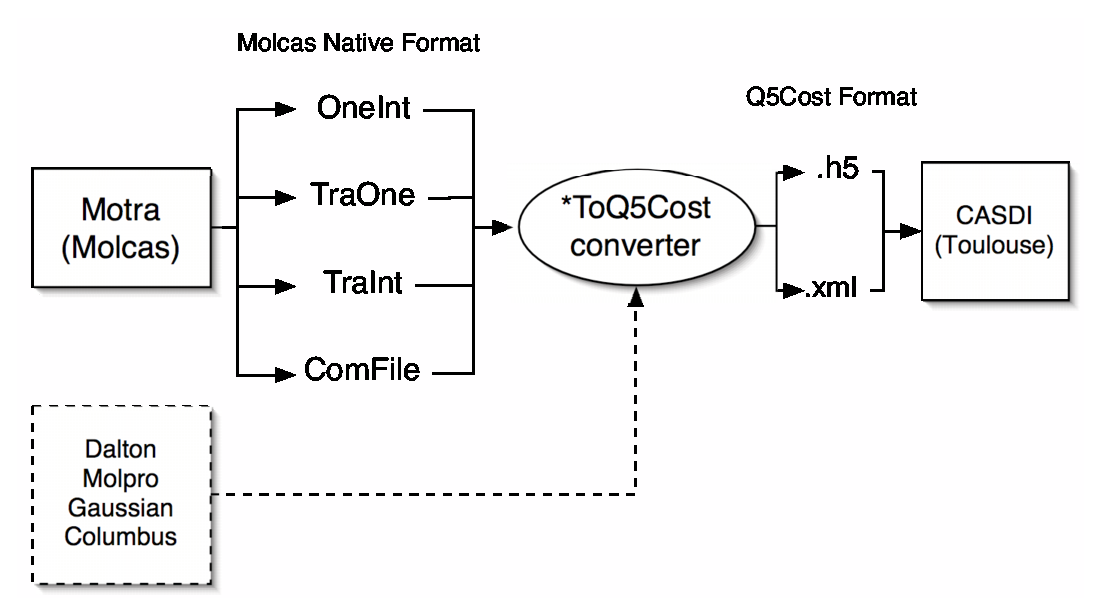
\includegraphics[width=10cm,keepaspectratio]{04_grid/images/q5cost-final-gimped.eps}
\end{center}
\caption{\footnotesize One of the possible final code layouts, involving
direct changes in the code. An integral producer, such as \texttt{MOLCAS}, provides
proprietary files. These files are fed to a converter, which creates the new
Q5Cost format. The program \texttt{CASDI} from Toulouse directly reads these
files. This infrastructure at the moment is not possible, because the
current \texttt{CASDI} implementation reads the old COST format.}
\label{fig:q5cost-final}
\end{figure}
\end{center}

Output integrals are produced by a commercial package, \molcas in the
example, but converters could be developed for other programs, like
\texttt{DALTON}, \texttt{COLUMBUS} and so on. These integrals are fed into a converter to
produce the Q5Cost file format, made of the HDF5 file and an XML (QCML) file
providing additional information. The Q5Cost format will be read by
CASDI, a program from the Toulouse chain of programs. This
approach assumes that \texttt{CASDI} is directly interfaced with the Q5Cost format. 

A more conservative way to handle this interface is represented in Fig.
\ref{fig:q5cost-intermediate}.
\begin{center}
\begin{figure}[ht]
\begin{center}
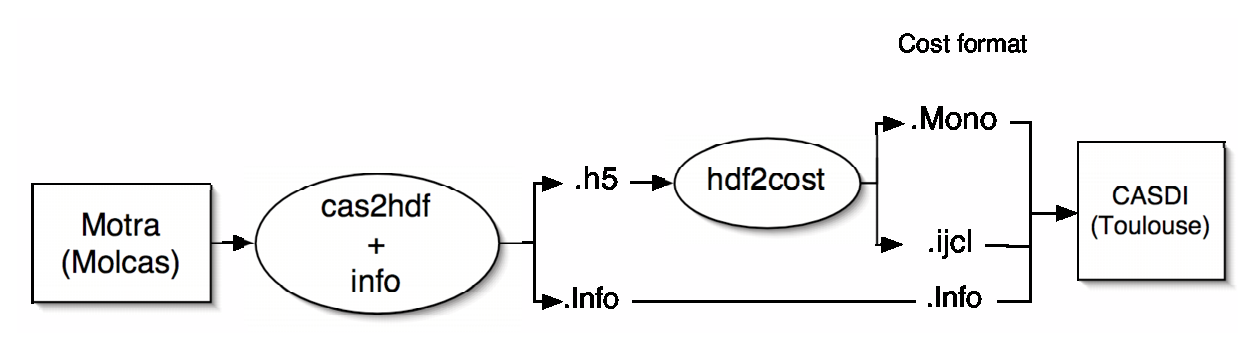
\includegraphics[width=10cm,keepaspectratio]{04_grid/images/q5cost-intermediate-gimped.eps}
\end{center}
\caption{\footnotesize A conservative solution. The \texttt{cas2hdf}
program produces the Q5Cost file, which is converted to the old COST format with
\texttt{hdf2cost}. The \texttt{.Info} file is used as a temporary
replacement of the XML file, and is provided by the \texttt{info}
program, directly interfaced with the \molcas suite. This solution does not
need changes in the CASDI code, and is therefore preferred in the initial
deployment. }
\label{fig:q5cost-intermediate}
\end{figure}
\end{center}

The \texttt{cas2hdf} program directly accesses the \molcas files, producing the
Q5Cost file. The \texttt{.Info} file is used as a temporary replacement of
the XML file, and it is provided by the \texttt{info} program.
The resulting Q5Cost file is read by \texttt{hdf2cost} and converted to the
old COST format, which can be directly read by CASDI.  This solution does
not need changes in the \texttt{CASDI} code, and is therefore preferred in the
initial deployment.

The deployment of these tools made possible to obtain a successful
interface between \molcas and \texttt{CASDI}. Some successful experiment has been also
performed with \texttt{DALTON}.

An experiment of direct integration has been performed with the
\texttt{Full-CI}\cite{cpl-252-437-1996,ijqc-48-287-2004} program developed
in the Professor Bendazzoli research group at Bologna University. The
\texttt{Full-CI} code is now able to read Q5Cost files, and can be
interfaced with both \molcas and \texttt{DALTON}.


\section{F77/F90xml library}

The Extensible Markup Language (XML) file format plays a central role in the
modern internet infrastructure. XML is derived by the more general format
Standard Generalized Markup Language (SGML), and is visually very similar to
HTML (the file format for web pages) although HTML itself is not a XML
document. 

The official definition provided by the W3 Consortium\cite{w3c-site} states
that the ``\textit{Extensible Markup Language (XML) is a simple, very flexible text
format derived from SGML (ISO 8879).  Originally designed to meet the
challenges of large-scale electronic publishing, XML is also playing an
increasingly important role in the exchange of a wide variety of data on the
Web and elsewhere}''.

The main advantages of this format are:
\begin{itemize}
\item internet standard, as accepted by the W3 Consortium
\item platform independent
\item clean and terse human readable textual format
\item very practical and extensible
\item can be checked for syntactical and semantical correctness
\item allows the description of data and their meaning
\item can be commented inline
\item already existent libraries for accessing the document
\end{itemize}

An example of an XML document is given below

\begin{verbatim}
<?xml version="1.0"?>
<book ISBN="0140390839">
 <!-- a comment -->
 <author>Mark Twain</author>
 <title>Tom Sawyer</title>
 <chapter>
  <title>First Chapter</title>
  This is the content of the first chapter.
 </chapter>
 <emptypage />
 <chapter>
  <title>Second Chapter</title>
  This is the content of the second chapter.
 </chapter>
</book>
\end{verbatim}

An XML document holds \textit{markup} and \textit{content}. The most common type of markup is
the \textit{Element}, delimited by angle brackets and normally present in pairs of
begin tag (for example ``\texttt{author}'') and end tag (the same tag name, but
prepended by a slash ``\texttt{/}'' symbol). These elements wrap content and other
markups in a nested parent/child relationship, defining a tree-like
structure. If an Element has no content, an alternative abbreviated syntax
can be used to represent the begin/end as a single tag. The
``\texttt{emptypage}'' Element is an example of such syntax.

Another kind of markup is the \textit{Attribute}. Attributes are name/value
pairs defined in the context of an Element. An example of this markup is the
``\texttt{ISBN}'' entry for the ``\texttt{book}'' Element.

Finally, a comment markup can be seen in the provided example.  Other kinds
of markups, such as processing instruction, entity references or CDATA
sections, will not be analyzed in this thesis.

Two constraints define the correctness of an XML document:
\begin{itemize}
\item \textit{well-formedness}
\item \textit{validity}
\end{itemize}

An XML document is well-formed if it complies with the XML specification.
Using square brakets instead of angular brakets is an example of non
well-formedness. Improper nesting of elements such as
\begin{verbatim}
 <author>Mark<Title>Twain</author>Tom Sawyer</title>
\end{verbatim}
is another example. XML Parsers must report an error when a non well-formed
document is provided.

Validity is related to well-formed documents that comply with a logical
meaning, related to the chosen data model. 
For example, the document
\begin{verbatim}
<?xml version="1.0"?>
<title>
 <book>
  Tom Sawyer
  <author ISBN="0140390839">
   <chapter>
    This is the content of the first chapter.
   </chapter>
  </author>
 </book>
</title>
\end{verbatim}
is a well-formed document, but has poor or no meaning in the analyzed data
model. Validity depends on the context and is defined by Document Type
Definitions, or XML-Schemas, which will not be detailed in this thesis. Pure
parsing cannot check for validity unless DTD or schemas are provided.

Accessing XML documents can be performed through two standardized interfaces:

\begin{itemize}
\item \textit{SAX}, Simple API for XML
\item \textit{DOM}, Document Object Model
\end{itemize}

SAX is an event-driven parser. While the document is read (from a file, or
from a network socket) the parser calls specific callback routines (handlers) to
process the current Element (start or stop markups), or Attribute, or
content (TextNode). Each handler is normally defined by the developer of the
client code, and expresses the contextual behavior related in finding a
certain Element, or TextNode.

SAX has some important advantages: first, parsing can be performed on a
partial document. This is very important if the document is very large, or
if the parsing must begin as soon as the first data are available. This
can produce a more pleasant experience of responsiveness to the user if, for
example, the document is downloaded from a slow network connection.

Second, the SAX parsing has a very small memory footprint. The document does
not need to be held in memory. Nodes can be parsed and discarded after the
event has been dispatched to the appropriate handler. This is very important
if the document is very large. 

SAX has also disadvantages: is a readonly parser (it can only read
documents, but cannot build and write an XML tree), is stateless, is purely
sequential, and finally is rather difficult to use. 

The other available parser is DOM. DOM is an interface to an
{Object Oriented} description of the XML document. The main advantage of DOM
is represented by the ability to handle the document in ways not provided by
SAX: DOM interface directly exposes the tree data abstraction in terms of
Nodes (\textit{flat interface}) or specialization of the Node concept, like Element,
Attribute, Document, TextNode, and so on (\textit{specialized interface}).
The document is parsed as a whole and a tree representation is built in
memory. This representation can be parsed, read and altered with a random
access approach, and finally written back to disk or to a network
connection. DOM interface is also simpler to use than SAX. 

The main drawback of DOM is the need to hold a complete representation of
the document in memory. For this reason, DOM parsing is generally not
applicable on partial or very large documents.

Two interface levels are available, and a third is almost ratified.
DOM Level 1 provides the basic handling of the tree. DOM Level 2 and 3
provide additional advanced features like namespacing and events. Only a
restricted set of Level 2 features are needed for the project.

\subsection*{XML and Fortran}

Calculations in scientific environments such as physics, chemistry,
astronomy and so on are still bound to the Fortran language.  Other
high-level languages such as C, C++, Java, Python are of difficult
deployment.  Techological problems (compatibility, library availability,
efficiency) human factors and historical reasons (learn new abstractions and
patterns, rewrite the legacy code) prevent a switch to other languages.

Of course, this is a strong limiting factor in keeping the pace with the
rapid evolution of network and computational resources. Using these new
technologies often requires dedicated middleware, specifically designed to
simplify access by wrapping low-level functionality with a high-level
interface. XML handling is an example of the reported situation: an XML
document is a plain text file, but its complex, extensible structure goes beyond
its pure textual nature. SAX and DOM parsers are high-level frontends to XML
document management, taking care of low-level issues and presenting a new
abstraction to the programmer.

The lack of a Fortran library to handle XML can be a problem when the
deployment of new standards is needed and the handling of these standards
must be performed by Fortran programmers, like in the case of the AbiGrid
project. Currently available libraries for XML access in Fortran are
``xml''\cite{xmllib-site} and {``xml-fortran''}\cite{xml-fortran-site}, 
not DOM compliant and written in pure Fortran, and ``xmlf90''
\cite{xmlf90-site} which supports SAX and DOM Level 1 and is written in the
F subset of Fortran.

Among the problems of these solutions are:

\begin{itemize}
\item non DOM Level 2 compliant (no namespaces support)
\item rather difficult to use and extend
\item read only
\item string handling is very rigid
\item bound to F90 compilers
\end{itemize}

The first five points are indeed critical. Deploying advanced features like
DOM or XPath (a standardized method to access Nodes using a syntax similar
to a filesystem path) is very difficult with a pure Fortran approach.
Fortran has limits in strings, file handling and object management.

The latter point is more controversial. Many commercial Fortran 90 compilers
exists. Some of them are available at no cost, but this policy could change
in the future. With the release of free Fortran 90 compilers like g95
\cite{g95-site} and gfortran \cite{gfortran-site}, the latter point is no
longer an issue, but was a prerequisite in the initial development of
F77/F90xml.

\section{F77/F90xml implementation}
% {{{
The F77/F90xml library \cite{f77f90xml-site} is a C library designed to
provide a Fortran interface to libgdome2 \cite{gdome2-site}, an opensource
library (also developed using C language) part of the GNOME
\cite{gnome-site} project. Most of the design is implemented to give access
to a DOM level 2 interface \cite{w3-dom-level-2-site}, with the exclusion of
events, which are not needed in the target environment. XPath support is
available, although no testing has been performed and therefore must be
considered experimental.

At the time of writing, F77/F90xml library depends on libgdome2-0.8.0,
glib-1.2.10 \cite{glib-site}, libxml2-2.5.11 \cite{libxml2-site}.  Building
of the library also depends on Python 2.3 \cite{python-site} or above.  The
library has been successfully compiled on Intel/AMD Linux platform, with gcc
and Intel Fortran Compiler, and IBM SP4 with the xlf compiler suite. It is
released under the terms of the LGPL \cite{lgpl-site}.

F77/F90xml has been designed with Fortran 77 backward compatibility in mind.
The library provides two interfaces: a Fortran 90/95 interface, similar to
DOM Level 2 in order to reduce the need for specialized documentation, and a
Fortran 77 interface, using specialized subroutines named
\textit{multiplexers}.

The Fortran 77 interface is particularly complex and error prone.  An
experimental preprocessor has been deployed to translate pseudo-F90 code
into F77 code, but Fortran 77 is very old and the choice for new code should
be Fortran 95. Support for this language was an initial request from the
interested parties, and provides full freedom even to those projects that
still work in a pure Fortran 77 environment for their maintenance. 

When the library development started, no stable and free Fortran 90/95
compiler existed, and most of the potentially interested parties had the
requisite to compile the code using the GNU F77 compiler.  This situation
changed with the release of g95 and gfortran, however the Fortran 77
interface is directly obtained from the implementation, simplifying rather
than making more difficult the development of the library.

In the following, we will refer to the Fortran 90 interface with the term
``F90xml'', and with ``F77xml'' to the specific Fortran 77 interface.
Finally, the term ``F77/F90xml'' refers to the library as a whole.
% }}}

\subsection*{The Fortran 90/95 interface}

The Fortran 90/95 interface provides a clean and simple access. All gdome2
functions are mapped to Fortran subroutines, collected together into a 
\texttt{MODULE}. A simple code example is provided 

{
\footnotesize
\begin{verbatim}
INTEGER :: first, last, elem, err

Comment <... get elem by some other call ...>

CALL f90xml_el_firstChild(first,elem,err)
CALL f90xml_el_lastChild(last,elem,err)
\end{verbatim}
}

which can be compared with the equivalent C code

{
\footnotesize
\begin{verbatim}
GdomeElement *elem;
GdomeNode *first, *last;
GdomeException exc;

/* <... get elem by some other call ...> */

first = gdome_el_firstChild(elem, exc);
last = gdome_el_lastChild(elem, exc);
\end{verbatim}
}

This comparison presents the main featured differences of the F90xml usage
with respect to gdome2. Apart of the routine names, where the standard
prefix ``\texttt{gdome\_}'' is replaced with ``\texttt{f90xml\_}'', two
major differences exist. 

The first difference is bound to the data reference handling.  The C
interface provided by gdome2 is structured in {Object Oriented} style.
Routines handle pointers to structures, dynamically allocated inside the
library. 

To prevent issues relative to the handling of memory pointers
between C and Fortran, the F77/F90xml library provides a simple mapping
between an integer value and a memory pointer (for example to
\texttt{GdomeNode}, \texttt{GdomeDOMString},
\texttt{GdomeDomImplementation}, and so on).  Fortran client code always
handle these integers, hereafter named
\textit{codes}, univocally identifying a particular gdome pointer.  The
F77/F90xml library internally implements a cache to store these pointers and
the corresponding code, providing an internal facility to obtain codes from
memory pointers and viceversa.  The current implementation of the library
uses a simple linked lists to store the mapping, and this correspondence is
kept until the gdome2 object is completely deallocated.  Substitution of the
linked list with a more efficient hash table can be implemented
transparently.

The second major difference is the arguments layout: in F90xml, the
first argument of the subroutine is the gdome2 returned value, therefore the
{Fortran~90} interface declares this argument as \texttt{INTENT(OUT)}. The
subsequent arguments are the requested gdome2 arguments, marked as
\texttt{INTENT(IN)} in the {Fortran~90} interface, with the
exception of the last one, holding the returning error condition and
therefore marked as \texttt{INTENT(OUT)}. 

If the gdome2 function returns \texttt{void} (no value), the corresponding
F90xml subroutine accepts an integer as a first argument. On return, this
value is set to the standard numeric parameter \texttt{NullCode}, which
evaluates to zero. 

\subsection*{String handling}

For most of the time, strings in F77/F90xml are handled as codes
representing \texttt{DOMString} objects: when an element name is requested,
the F77/F90xml subroutine returns a code referencing a \texttt{DOMString}
object. Setting an element name or TextNode data requires passing a
\texttt{DOMString} code. A set of routines has been provided to simplify the
handling of these objects:
\begin{itemize}
\item \texttt{f90xml\_str\_mkref}: creates a new \texttt{DOMString} from a Fortran
\texttt{CHARACTER} string. Accepts the Fortran string and returns a code referencing
the newly created \texttt{DOMString} object.
\item \texttt{f90xml\_str\_length}: accepts the code of the \texttt{DOMString} and
returns the length of the string.  This routine can be useful to know in
advance how many bytes are needed to read from the \texttt{DOMString}, and act
accordingly. A classical example could be a \texttt{DOMString} containing 300 bytes
and the Fortran code has a \texttt{CHARACTER(LEN=100)} available.
\item \texttt{f90xml\_str\_toFortran}: extracts Fortran character
data from an existing \texttt{DOMString} object. This routine accepts the code of the
\texttt{DOMString}, a \texttt{CHARACTER(LEN=*)} variable, an \texttt{INTEGER} offset
and returns a \texttt{LOGICAL} value. The \texttt{DOMString} data will be extracted
starting at the position provided by the zero-based offset. No more than
the length of the \texttt{CHARACTER} variable will be extracted from the
\texttt{DOMString}. The returned \texttt{LOGICAL} value is set to \texttt{.TRUE.} if the
\texttt{DOMString} has been extracted up to the last character, otherwise
\texttt{.FALSE.}. Using the returned logical value and working with
appropriate offsets, it is possible to read long strings in a chunked
fashion, regardless of the effective dimensions of the \texttt{DOMString} and
\texttt{CHARACTER} variable.
\item \texttt{f90xml\_str\_print}: Prints the \texttt{DOMString} to standard
output. Returns \texttt{void}. 
\item \texttt{f90xml\_str\_equal}: Performs a comparison between
a \texttt{DOMString} referenced by its code and a Fortran \texttt{CHARACTER} string.
Returns \texttt{.TRUE.} if the strings are equal, otherwise \texttt{.FALSE.}
\item \texttt{f90xml\_str\_unref}: deletes the \texttt{DOMString}. Returns
\texttt{void}.
\end{itemize}

\subsection*{Errors}

The F77/F90xml library returns the error status \textit{via} the last
\texttt{INTEGER} argument. The returned value depends on the kind of error,
and a list of \texttt{PARAMETER}s account for all the available situations.
The \texttt{ERR\_NO\_ERROR} value, which evaluates zero, is returned if no
error occurs. The library checks for various error conditions, such as
\begin{itemize}
\item a passed code is not of the expected type, after inquiry into the cache
(e.g. passing the code corresponding to \texttt{DOMString} to
\texttt{f90xml\_el\_firstChild})
\item a code does not reference to any cached object
\item a \texttt{NullCode} is passed to a routine unable to handle it
\item internal errors of the gdome2 library
\end{itemize}

\subsection*{Library architecture and Fortran 77 interface}

Standard Fortran 77 expects names limited to 6 characters, although at our
knowledge no recent Fortran 77 compiler imposes this strict limit. Deploying
the complete DOM interface with a one-to-one mapping in such limited
namespace would result in name collisions and routine names with no meaning.

To face this issue, a few multipurpose C functions have been created, named
\textit{multiplexers}.  The role of each multiplexer is to create a
many-to-one correspondence between a subset of the gdome2 routines accepting
the same number and type of arguments and the single generic multiplexer
function. Multiplexers give access to the complete interface with a reduced
namespace footprint.

Each C multiplexer is directly mapped by the library to a F77
\texttt{SUBROUTINE}, in a one-to-one relationship.  Code between the Fortran
frontend and the corresponding C multiplexer is needed to interface these
two languages and their different standards for string handling, memory
management, routine name mangling and parameters. 

The multiplexers are the core of the library. When a multiplexer is
called, it dispatches (demultiplexes) the call to the appropriate function
of the subset it describes. In turn, this function performs the actual call
to the gdome2 routine. To select which routine to call, a string containing
the name of the routine is passed as an argument. Internally, this information
is used to invoke the correct function.  Fig. \ref{fig:f77xml-high-level}
represents a high-level view of a single multiplexer. 

Each multiplexer routine and its Fortran interface have a standardized name,
bound to the number and type of arguments it accepts.

A schematic classification of the routines has been devised to describe with
a short notation the number and type of accepted parameters, and the
returned value.  Routines with the same type signature are handled by the
same multiplexer.  The core implementation resorts on the equality of
signatures to collect pointers to functions. 

In the following, a textual representation of the signature will be written
in the compact form \texttt{(return|arguments)}.  For each kind of argument,
a letter has been assigned: ``\texttt{c}'' for code, ``\texttt{b}'' for
boolean (logical), ``\texttt{e}'' for error, ``\texttt{s}'' for string,
``\texttt{u}'' for unsigned integer.  Also, the ``\texttt{v}'' is used with
subroutines that return no value (are \texttt{void} in C syntax). 

As an example, all the gdome2 functions given below

{
\footnotesize
\begin{verbatim}
GdomeNode* gdome_el_firstChild(GdomeElement *self, GdomeException *exc);

GdomeElement* gdome_doc_documentElement(GdomeDocument *self, GdomeException *exc);

GdomeNode* gdome_el_lastChild(GdomeElement *self, GdomeException *exc);
\end{verbatim}
}
accept a code and an error and return a code. The signature of these
functions therefore is \texttt{(c|ce)} and they are handled by the
same multiplexer.  The associated Fortran entry point is the subroutine
\texttt{xp3t1}, where ``\texttt{x}'' is a standard prefix, ``\texttt{p3}''
(literally ``parameters 3'') denotes the number of arguments involved in the
signature (two codes and the error) and ``\texttt{t1}'' (literally, ``type
1'') is bound to the type of the arguments.  The type is needed to
distinguish routines that accept 3 parameters of a different type.  For
example, the following routine 
\begin{center}
\begin{figure}[t]
\begin{center}
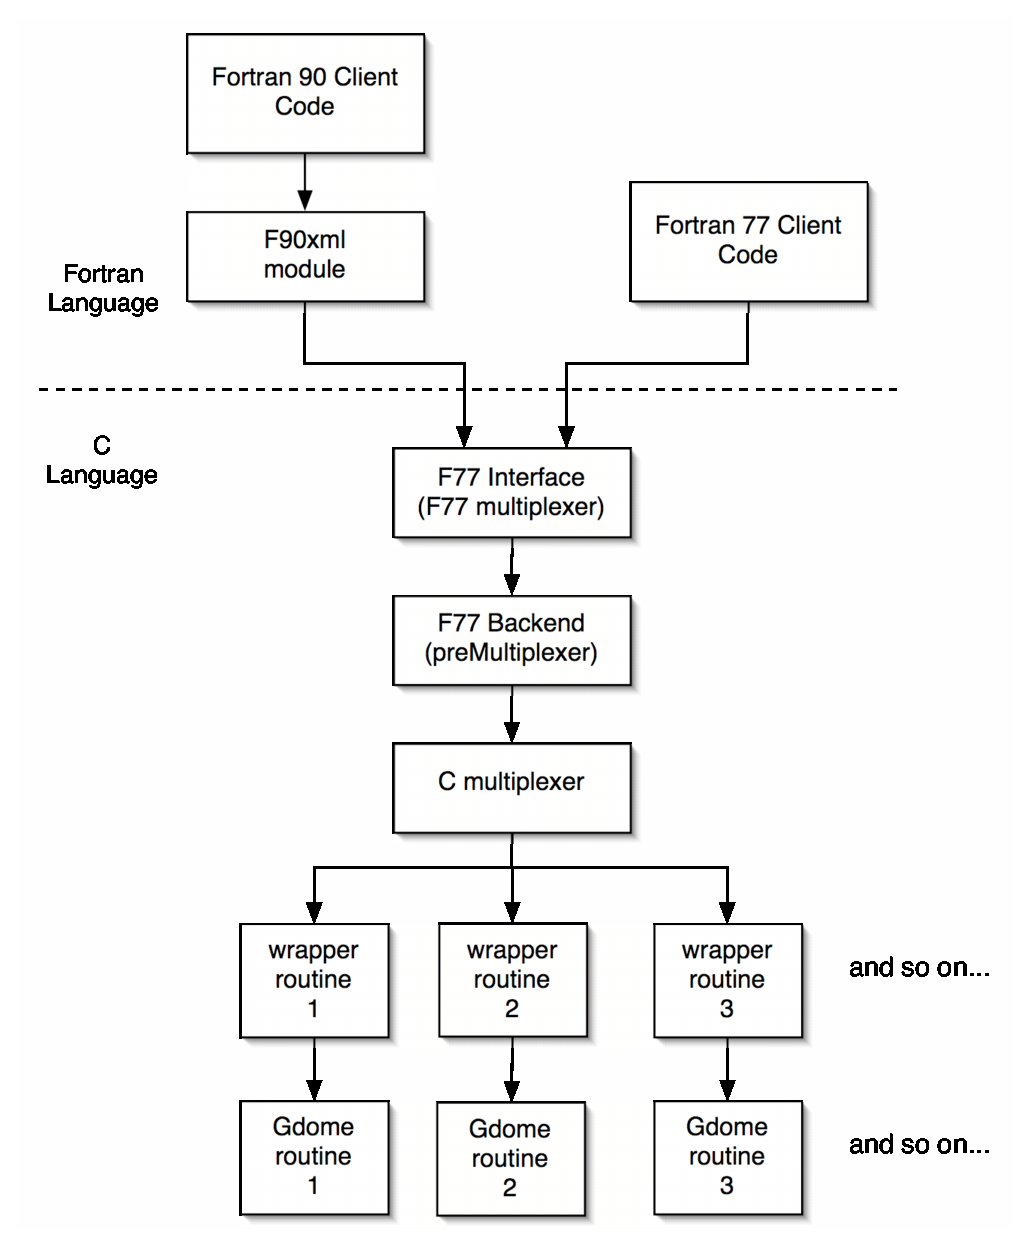
\includegraphics[width=100mm,keepaspectratio]{04_grid/images/f77xml-high-level-gimped.eps}
\end{center}
\caption{\footnotesize A graphical scheme representing the F77/F90xml
library structure. Each multiplexer groups a high number of gdome2
subroutines.}
\label{fig:f77xml-high-level}
\end{figure}
\end{center}

{
\footnotesize
\begin{verbatim}
GdomeBoolean gdome_el_hasChildNodes(GdomeElement *self, GdomeException *exc);
\end{verbatim}
}
has signature \texttt{(b|ce)} and is handled by a multiplexer with the same
\texttt{p} value but different \texttt{t} value: \texttt{xp3t4}

An exception is represented by routines returning \texttt{void},
\texttt{(v|ce)}. These routines are handled as \texttt{(c|ce)} routines,
accepting a dummy return argument which is set to the special value
\texttt{NullCode}. In other terms, both \texttt{(c|ce)} and \texttt{(v|ce)}
routines are managed by the same multiplexer, the \texttt{xp3t1} multiplexer.
It must be pointed out that no matching scheme exists to obtain the type
number from the letter sequence in the signature. 

The \texttt{xp3t1} multiplexer by itself maps and gives access to
approximatively 240 gdome2 functions. The complete DOM interface (more than
450 functions) is mapped by 21 multiplexers. As already said, the
gdome routine is chosen by the means of a \texttt{CHARACTER} argument which
is passed to the multiplexer.  By convention, this argument is passed
between the return value and the first \texttt{INTENT(IN)} argument,
therefore always in the second position. 

As a final result, the Fortran 77 interface to the multiplexer is
represented in the example below

{
\footnotesize
\begin{verbatim}
       CHARACTER*128 fnName
       INTEGER first, last , elem, err

Comment <... get elem by some other call ...>

       fnName='el_firstChild'
       CALL xp3t1(first,fnName,elem,err)

       fnName='el_lastChild'
       CALL xp3t1(last,fnName,elem,err)
\end{verbatim}
}
As can be seen from the example, the function name is case sensitive and is
the exact copy of the gdome2 function, stripped of the ``\texttt{gdome\_}''
prefix.  The Fortran 90 module provides long named subroutines performing
the mapping between each subroutine and the corresponding multiplexer.

The library architecture here presented was chosen for two reasons: 
\begin{itemize}
\item reduce the development cost, providing automatized creation of the
library
\item keep potential Fortran 77 compatibility.
\end{itemize}

A large part of the library is developed in XML. An XML file contains all
the informations to create the binding routines called from the C
multiplexers.  The file is parsed by a Python script which
collects the needed informations, and deploys the C and Fortran code. 

The logic involved is to define templates for the binding routines, and to
replace ad-hoc placeholder keywords with appropriate entries for the
specific routine. When a particular specific implementation cannot be
generated by a template, the format allows to override the template
mechanism and to pass the specific implementation.

We can note that the Fortran 77 interface is a direct subproduct of the
internal implementation of the library, therefore is convenient to deploy it
even if not used by client code. 

%In order to simplify the cleanup of the allocated structures, the
%\textt{f90xml_cache_flush} routine is provided. Using this routine the
%client code can delay the cleanup of many objects to a single final call.
%Functions for unreferencing single structures (Nodes, DOMStrings etc...) are
%also available at F77/F90xml level.
%
%{
%\footnotesize
%\begin{verbatim}
%CHARACTER(LEN=4) :: fortranString
%\end{verbatim}
%}
%
%and accessing the \texttt{f90xml\_str\_toFortran} routine with fortranString and
%offset 0, fortranString will contain "Here" and the returned logical value will
%be \texttt{.FALSE.}. With an offset of 5, fortranString will contain "is t", and
%again the returned logical value will be \texttt{.FALSE.}. Finally, with an offset
%of 13, fortranString will contain "ata" and the returned logical value will
%be \texttt{.TRUE.}. 
%{
%\footnotesize
%\begin{verbatim}
%0 : ERR_NO_ERROR 
%\end{verbatim}
%}
%
%
%{
%\footnotesize
%\begin{verbatim}
%10 : ERR_DATA_NOT_AN_ELEMENT 
%11 : ERR_DATA_NOT_A_NODE  
%12 : ERR_DATA_NOT_A_DOCUMENT 
%13 : ERR_DATA_NOT_A_STRING  
%14 : ERR_DATA_NOT_A_NODELIST 
%15 : ERR_DATA_NOT_A_COMMENT  
%16 : ERR_DATA_NOT_AN_ATTR 
%17 : ERR_DATA_NOT_A_NAMEDNODEMAP 
%18 : ERR_DATA_NOT_A_TEXT     
%19 : ERR_DATA_NOT_AN_ENTITYREF  
%20 : ERR_DATA_NOT_AN_ENTITY 
%21 : ERR_DATA_NOT_A_PROCESSINGINSTRUCTION  
%22 : ERR_DATA_NOT_A_CDATASECTION 
%23 : ERR_DATA_NOT_A_DOCUMENTFRAGMENT
%24 : ERR_DATA_NOT_A_DOCUMENTTYPE   
%25 : ERR_DATA_NOT_A_DOMIMPLEMENTATION  
%\end{verbatim}
%}
%
%These errors are returned every time a passed code is not of the expected type, after inquiry into the cache.
%For example passing the code that corresponds to a DOMImplementation to
%f90xml\_el\_firstChild, a ERR\_DATA\_NOT\_AN\_ELEMENT is returned, because f90xml\_el\_firstChild expects an element.
%It is important to note that a code referring to an Element can be passed to Node handling
%subroutines like f90xml\_n\_appendChild (which accept a code for a node),
%because in the DOM abstraction an Element is a specialization of a Node.
%
%{
%%\footnotesize
%\begin{verbatim}
%30 : ERR_NO_CACHE_HIT
%\end{verbatim}
%}
%
%This error is returned when a given code does not reference to any object in
%the cache. This usually is indicative of a bug in the client code.
%
%{
%\footnotesize
%\begin{verbatim}
%31 : ERR_NULL_CODE
%\end{verbatim}
%}
%
%This error is returned when a NullCode is passed to a routine unable to
%handle it.
%
%{
%\footnotesize
%\begin{verbatim}
%1000 : ERR_NEVER_RETURN_THIS
%\end{verbatim}
%}
%
%A watchdog error value. No routine should return this error. If this
%happens, a library bug is the cause.
%
%{
%\footnotesize
%\begin{verbatim}
%10000: ERR_GDOME
%\end{verbatim}
%}
%
%An error at gdome2 level has been detected. A F77/F90xml library bug can
%trigger this error.


